\documentclass[aspectratio=169]{beamer}

\usetheme{default}
\usepackage[utf8]{inputenc}
\usepackage[brazil]{babel}
\usepackage{tikz}
\usepackage{tabularx}
\usetikzlibrary{positioning,shapes.geometric,arrows.meta}
\usepackage{amsmath}
\usepackage{booktabs}
\usepackage{multirow}
\usepackage{graphicx}
\usepackage{hyperref}
\usepackage{amssymb}
\usepackage{colortbl}
\newcolumntype{L}[1]{>{\raggedright\arraybackslash}p{#1}}

% logos em presentation/imgs; figuras desta apresentação em ./figuras
\graphicspath{{../}{figuras/}}

\setbeamertemplate{footline}[frame number]
\setbeamertemplate{frametitle}[default][center]

\mode<presentation>{
\usetheme{Dresden}
\usecolortheme{seagull}
}

\setbeamertemplate{headline}{}

\definecolor{peeblue}{RGB}{1,123,165}
\definecolor{darkblue}{RGB}{0,65,115}
\definecolor{lightgray}{RGB}{240,240,240}
\definecolor{goldencolor}{RGB}{190,140,0}
\definecolor{greenwin}{RGB}{0,130,50}

\setbeamercolor*{palette primary}{fg=black,bg=peeblue!80}
\setbeamercolor*{palette secondary}{fg=black,bg=peeblue!80!gray!80}
\setbeamercolor*{palette tertiary}{fg=black,bg=peeblue!100}
\setbeamercolor*{palette quaternary}{fg=black,bg=peeblue!110}

\usebackgroundtemplate
{%
    \begin{picture}(210,40)(-5,2)
    
\includegraphics[width=0.07\paperwidth,keepaspectratio]{imgs/pee-logo-short.png}
    \end{picture}%
}

\title{Reconhecimento Acústico de Alvos Submarinos no Dataset IARA}
\subtitle{Análise Exploratória: Por Que os Modelos Erram}
\author{Evandro Rocha}
\date{Novembro de 2026}

\institute
{
  Universidade Federal do Rio de Janeiro\\
  UFRJ / COPPE / PEE
}

\newcommand{\cahi}[1]{\cellcolor{green!30}\textbf{#1}}
\newcommand{\calo}[1]{\cellcolor{red!20}#1}
\newcommand{\camd}[1]{\cellcolor{yellow!35}#1}

\begin{document}

%===========================================
% CAPA
%===========================================
{
\usebackgroundtemplate{
    \begin{picture}(210,55)(-5,0)
    
\includegraphics[height=0.14\paperwidth,keepaspectratio]{imgs/pee-logo.png}
    \end{picture}%
    \begin{picture}(210,55)(-28,2)
    
\includegraphics[height=0.14\paperwidth,keepaspectratio]{imgs/coppe-logo.pdf}
    \end{picture}
}
\begin{frame}
  \bigskip\bigskip\bigskip\bigskip
  \titlepage
\end{frame}
}

%===========================================
% AGENDA
%===========================================
\begin{frame}{Agenda da Apresentação}
  \footnotesize
  \setbeamercolor{block title}{bg=darkblue,fg=white}
  \setbeamercolor{block body}{bg=peeblue!8,fg=black}
  \setbeamertemplate{section in toc}{%
    \vspace{0.14cm}%
    \leavevmode%
    \tikz[baseline=-0.65ex]\node[circle,fill=peeblue,text=white,inner sep=0pt,font=\tiny\bfseries,minimum size=1.35em]{\inserttocsectionnumber};%
    \hspace{0.35em}%
    \inserttocsection\par%
  }
  \begin{columns}[t]
      \begin{column}{0.48\textwidth}
          \begin{block}{\small\textbf{I. O Que Separa as Classes}}
              \tableofcontents[sections={1-4}]
          \end{block}
      \end{column}
      \begin{column}{0.48\textwidth}
          \begin{block}{\small\textbf{II. O Que Não Separa, e Por Quê}}
              \tableofcontents[sections={5-7}]
          \end{block}
      \end{column}
  \end{columns}
\end{frame}

\begin{frame}{Resumo em Uma Página}
    \footnotesize
    \begin{block}{\small Pergunta (Tarefa 1, reunião de 26/10)}
        \scriptsize
        Quais frequências são comuns a cada classe, e as gravações que os modelos erram têm o padrão de outra classe?
    \end{block}
    \begin{columns}[t]
        \column{0.49\textwidth}
        \begin{block}{\small O que encontrei}
            \scriptsize
            \begin{itemize}
                \setlength{\itemsep}{1pt}
                \item As LARGE acertadas têm uma \textbf{banda larga em 31--86 Hz}; as erradas não. Confirmei a banda em navios novos (200/200 divisões).
                \item A banda é uma \textbf{pista do modelo para LARGE}, mas aparece também em 43\% das SMALL e 35\% das MEDIUM: explica boa parte dos erros nas três classes.
                \item No DEMON, encontrei a pista equivalente: um \textbf{pico de modulação forte e grave}.
            \end{itemize}
        \end{block}
        \column{0.49\textwidth}
        \begin{block}{\small O que não encontrei}
            \scriptsize
            \begin{itemize}
                \setlength{\itemsep}{1pt}
                \item Não encontrei \textbf{nenhuma diferença acústica entre SMALL e MEDIUM} (nem entre Offshore Supply Ships e rebocadores) em LOFAR, MEL, DEMON, HHT ou espectro até 24 kHz.
                \item Verifiquei que o recall de MEDIUM ($\sim$60\%) vem sobretudo de \textbf{reconhecer navios repetidos} no treino e no teste; com split por navio, fica em 23--41\% (acaso: 25\%).
            \end{itemize}
        \end{block}
    \end{columns}
\end{frame}

%===========================================
% SEÇÃO 1: MÉTODO
%===========================================
\section{Método e Dados}

\begin{frame}
    \centering
    \huge Método e Dados
\end{frame}

\begin{frame}{O Dataset e a Validação Cruzada}
    \begin{columns}[t]
        \column{0.49\textwidth}
        \begin{block}{\small Coleção OS do IARA}
            \scriptsize
            1.706 gravações a 48 kHz, 586 navios.
            \vspace{0.05cm}

            \centering
            \begin{tabular}{llc}
            \toprule
            Subconj. & Passagem & Gravações \\
            \midrule
            A & perto ($\leq$ 250 m), com CPA & 456 \\
            B & perto ($\leq$ 250 m), sem CPA & 199 \\
            C & longe (250--500 m), com CPA & 341 \\
            D & longe (250--500 m), sem CPA & 449 \\
            E & fundo (sem navio) & 261 \\
            \bottomrule
            \end{tabular}
            \vspace{0.05cm}

            \raggedright
            Classes pelo comprimento: SMALL $<$ 50 m (476), MEDIUM 50--100 m (397), LARGE $\geq$ 100 m (572), BACKGROUND (261).
        \end{block}
        \column{0.49\textwidth}
        \begin{block}{\small Treino e teste (pipeline do artigo)}
            \scriptsize
            \begin{itemize}
                \setlength{\itemsep}{1pt}
                \item \textbf{5$\times$2 = 10 folds}, estratificados por classe.
                \item Em cada fold: treino 50\%, validação 12,5\%, teste 37,5\%.
                \item Split \textbf{por gravação}: o mesmo navio pode estar no treino e no teste.
                \item Usa \textbf{120 s por gravação}: CPA $\pm$ 60 s em A e C; os primeiros 120 s em B, D e E.
            \end{itemize}
        \end{block}
    \end{columns}
\end{frame}

\begin{frame}{Extração: LOFAR e MEL}
    \centering
    \scriptsize
    \renewcommand{\arraystretch}{1.1}
    \begin{tabular}{L{1.9cm}L{5.6cm}L{4.3cm}}
    \toprule
    Etapa & \textbf{LOFAR} & \textbf{MEL} \\
    \midrule
    Pré-processo & Remoção da média & Divisão pelo máximo de $|x|$ \\
    Decimação & \multicolumn{2}{L{10.1cm}}{$\times$3: 48 $\to$ \textbf{16 kHz}. Chebyshev I de ordem 8, corte em 6,4 kHz, \texttt{filtfilt} (fase zero) e reamostragem por FFT} \\
    Janela & \multicolumn{2}{L{10.1cm}}{Hann de 2.048 amostras (0,128 s), sem sobreposição: resolução de \textbf{7,8 Hz}} \\
    Espectro & $|X|$ em 20$\log_{10}$: \textbf{1.024 faixas}, 7,8 Hz a 8 kHz & Potência em \textbf{256 filtros mel}, 0--8 kHz; 10$\log_{10}$ relativo ao máximo da gravação (piso $-80$ dB) \\
    Fundo & TPSW na frequência (n = 21, p = 4, a = 2: janela de $\pm$164 Hz, lacuna central de $\pm$23 Hz); valores abaixo de $-0{,}2$ viram 0 & --- \\
    Integração & \multicolumn{2}{L{10.1cm}}{Média de 4 quadros (em dB): \textbf{uma linha a cada 0,512 s}} \\
    Normalização & \multicolumn{2}{L{10.1cm}}{Por linha: min--max para [0, 1], depois norma L2} \\
    Entrada da CNN & 32 linhas $\times$ 1.024 (16,4 s), passo de 16 linhas (8,2 s): 13 imagens por gravação & 32 linhas $\times$ 256, mesmo passo \\
    \bottomrule
    \end{tabular}
    \vspace{0.15cm}

    {\tiny Fonte: \texttt{src/iara/processing/analysis.py} e \texttt{default.py}. O TPSW (\textit{two-pass split window}) estima o fundo local de cada quadro e o subtrai; a lacuna central impede que uma raia eleve o próprio fundo.\par}
\end{frame}

\begin{frame}{Extração: DEMON e HHT}
    \centering
    \scriptsize
    \renewcommand{\arraystretch}{1.1}
    \begin{tabular}{L{1.9cm}L{5.1cm}L{4.8cm}}
    \toprule
    Etapa & \textbf{DEMON} & \textbf{HHT} \\
    \midrule
    Pré-processo & Passa-banda \textbf{1--2 kHz} no sinal de 48 kHz (Chebyshev II de ordem 6, causal) & Decimação $\times$24: 48 $\to$ \textbf{2 kHz} (FIR, fase zero); z-score da gravação \\
    Demodulação & $|x|$ (retificação de onda completa): fica o envelope da cavitação & --- \\
    Decimação & $\times$960 (80 $\times$ 12, FIR): 48 kHz $\to$ \textbf{50 Hz} & (no pré-processo) \\
    Análise & STFT com Hann de 512 amostras (\textbf{10,24 s}), passo de 5,12 s & Segmentos de \textbf{2,56 s a cada 5,12 s}; \textbf{EMD} com 8 IMFs; Hilbert: amplitude e frequência instantâneas \\
    Saída & Magnitude em \textbf{253 faixas de 0,098 Hz}, 0,39--25 Hz (sem log nem TPSW) & 1D: energia em 256 faixas de 1--1.000 Hz. 2D: 32 $\times$ 128 (80 ms $\times$ 7,9 Hz), em log \\
    Modelo & BiGRU: 15 quadros (76,8 s), passo de 5 quadros; padronização por faixa & --- \\
    \bottomrule
    \end{tabular}
    \vspace{0.15cm}

    {\tiny O DEMON mede \textbf{a que ritmo} o ruído de cavitação pulsa (rotação do eixo $\times$ número de pás), não o espectro do ruído. No NB36, aplico TPSW (em 20$\log_{10}$) sobre o DEMON. Na HHT, metade do sinal não é usada (segmentos de 2,56 s com passo de 5,12 s). Diferente do pipeline do artigo, DEMON e HHT usam a gravação inteira.\par}
\end{frame}

\begin{frame}{Como Comparei Gravações Acertadas e Erradas}
    \footnotesize
    \begin{columns}[t]
        \column{0.49\textwidth}
        \begin{block}{\small Rótulos de acerto e erro}
            \scriptsize
            \begin{itemize}
                \setlength{\itemsep}{1pt}
                \item Usei como referência a \textbf{CNN LOFAR do artigo} (SP 66,5\%). Cada gravação é teste em $\sim$5 dos 10 folds.
                \item \textbf{Acertada}: acerta em todos os folds; \textbf{errada}: erra em todos; \textbf{oscila}: o resto (fora do contraste).
                \item Separei as erradas pelo \textbf{destino} (classe prevista na maioria dos folds).
                \item Para robustez, repeti com o consenso CNN + MLP + SVM LOFAR (perfil igual, $r = 0{,}995$).
            \end{itemize}
        \end{block}
        \column{0.49\textwidth}
        \begin{block}{\small Estatística}
            \scriptsize
            \begin{itemize}
                \setlength{\itemsep}{1pt}
                \item Usei o \textbf{navio como unidade} (média das suas gravações), para que navios muito gravados não pesem mais.
                \item Apliquei Mann-Whitney faixa a faixa, com FDR de Benjamini-Hochberg.
                \item \textbf{AUC} = P(errada $>$ acertada); 0,5 = sem diferença; 0,12 = forte diferença no sentido oposto.
                \item Validei em \textbf{metades de navios}: escolho a faixa numa metade e meço na outra.
            \end{itemize}
        \end{block}
    \end{columns}
    \vspace{0.05cm}
    {\scriptsize Usei o \textbf{LOFAR sem normalização} (dB acima do fundo TPSW) e o \textbf{espectro médio da gravação inteira}; a CNN vê o mesmo LOFAR, normalizado por linha e só nos 120 s centrais. Abaixo de $\sim$150 Hz o TPSW tem efeito de borda: a \textbf{comparação entre grupos} continua válida.\par}
\end{frame}

\begin{frame}{Extrações Novas que Criei Para Esta Análise}
    \footnotesize
    \begin{table}
    \centering
    \scriptsize
    \begin{tabular}{p{2.6cm}p{6.2cm}p{4.2cm}}
    \toprule
    \textbf{Nome} & \textbf{O que é} & \textbf{Para quê} \\
    \midrule
    \texttt{lofar1hz} & LOFAR com decimação para 2 kHz e FFT de 2048: faixas de 0,98 Hz (8$\times$ mais finas), mesmo passo de 0,512 s e TPSW com a mesma largura em Hz & Separar banda larga de raias estreitas próximas \\
    \texttt{psd24k} & Espectro de Welch do áudio original de 48 kHz, 0--24 kHz, sem decimação e sem normalização (blocos de 10 s) & Alta frequência (o LOFAR para em 8 kHz) e nível \\
    \texttt{demon\_multibanda} & DEMON em 0,5--1, 1--2, 2--4, 4--8 e 8--16 kHz (o do projeto usa só 1--2 kHz, reproduzido exatamente) & Modulação em outras bandas de cavitação \\
    \bottomrule
    \end{tabular}
    \end{table}
    \vspace{0.05cm}
    {\scriptsize Scripts em \texttt{scripts/extrair\_*.py}; saídas em \texttt{data/iara\_processed/}. Dei nomes distintos para não confundir com as representações do pipeline.\par}
    \vspace{0.1cm}
    {\scriptsize\textbf{Notebooks que produzi:} NB35 (LOFAR: LARGE, MEDIUM, SMALL), NB36 (DEMON: idem), NB37 (OSS $\times$ rebocadores em representações novas), NB38 (classificador com split por navio).\par}
\end{frame}

%===========================================
% SEÇÃO 2: LARGE
%===========================================
\section{LARGE: a Banda de 31--86 Hz}

\begin{frame}
    \centering
    \huge LARGE: a Banda de 31--86 Hz
\end{frame}

\begin{frame}{O Que É uma Banda Larga}
    \centering
    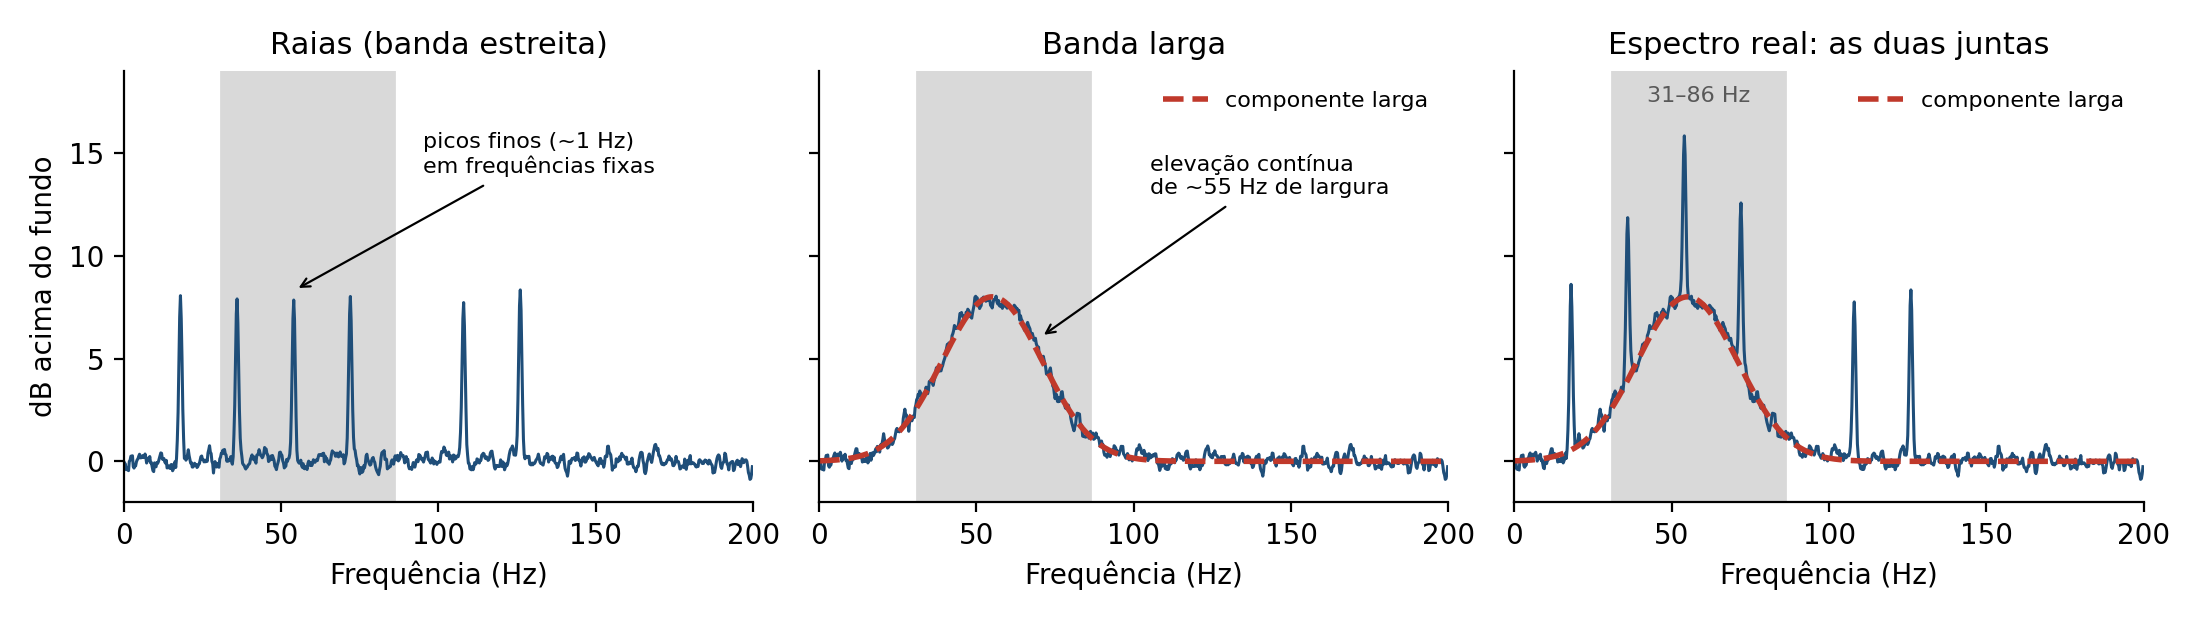
\includegraphics[width=0.9\textwidth]{banda_larga_esquema.png}

    {\tiny Esquema ilustrativo (dados sintéticos). Faixa cinza: 31--86 Hz. \textcolor{red}{Tracejado}: mediana móvel, que apaga as raias e deixa só a componente larga.\par}
    \vspace{0.05cm}
    \begin{columns}[t]
        \column{0.49\textwidth}
        \begin{block}{\small Raias (banda estreita)}
            \scriptsize
            Picos finos (1--2 Hz) em frequências exatas, do que gira ou pulsa em ritmo fixo: eixo, pás da hélice, motor. No LOFAR, linhas verticais finas.
        \end{block}
        \column{0.49\textwidth}
        \begin{block}{\small Banda larga}
            \scriptsize
            Energia contínua numa faixa, sem pico definido: cavitação, turbulência, escoamento. No LOFAR, uma faixa difusa. ``Larga'' em relação às raias ($\sim$50$\times$ mais larga).
        \end{block}
    \end{columns}
    \vspace{0.05cm}
    {\scriptsize A seguir, ``a banda'' é uma elevação contínua em 31--86 Hz, com pico perto de 55 Hz.\par}
\end{frame}

\begin{frame}{LARGE Acertadas Têm uma Corcova Grave}
    \centering
    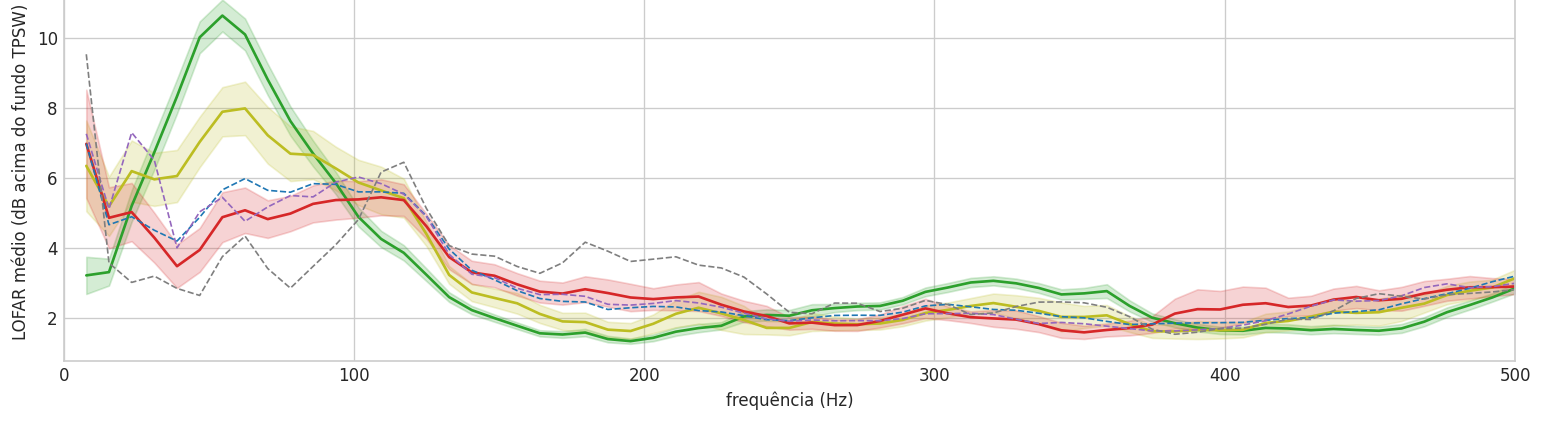
\includegraphics[width=0.92\textwidth]{lofar_large_espectro_zoom.png}

    {\tiny Espectro LOFAR médio, 0--500 Hz (faixa = IC 95\%). \textcolor{greenwin}{Verde}: LARGE acertadas (346); \textcolor{goldencolor}{amarelo}: oscilam (109); \textcolor{red}{vermelho}: erradas (117). Tracejadas: SMALL (azul), MEDIUM (roxo), BACKGROUND (cinza).\par}
    \vspace{0.05cm}
    \begin{alertblock}{Leitura}
        \scriptsize
        Acertadas: pico em 55 Hz, 10,7 dB acima do fundo; erradas: 4,9 dB. Maior diferença: $-6{,}4$ dB em 47 Hz (AUC 0,11). Em 0--500 Hz, as LARGE erradas estão a 0,36 dB (RMS) do espectro médio de SMALL, contra 1,53 dB das acertadas. A diferença aparece \textbf{dentro de cada subconjunto} A--D (p $<$ 0,001 em todos).
    \end{alertblock}
\end{frame}

\begin{frame}{Onde Fica o Pico Grave de Cada Gravação}
    \centering
    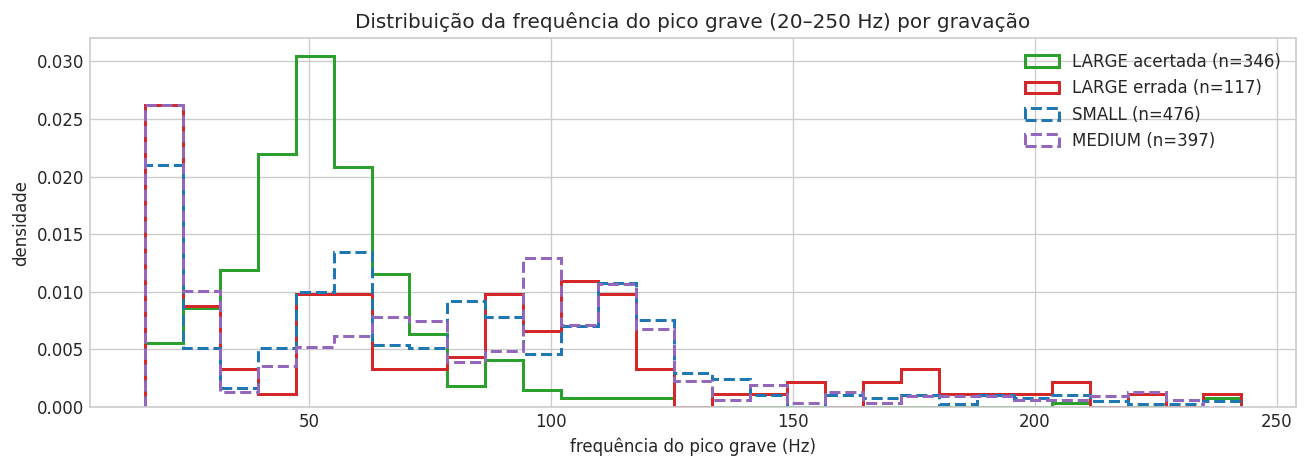
\includegraphics[width=0.85\textwidth]{lofar_large_pico.png}
    \vspace{0.05cm}
    \begin{columns}[t]
        \column{0.49\textwidth}
        \begin{block}{\small Pico grave em 31--86 Hz}
            \scriptsize
            \centering
            \begin{tabular}{lc}
            \toprule
            LARGE acertadas & \textbf{88\%} \\
            LARGE erradas & 34\% \\
            SMALL (todas) & 43\% \\
            MEDIUM (todas) & 35\% \\
            \bottomrule
            \end{tabular}
        \end{block}
        \column{0.49\textwidth}
        \begin{block}{\small É uma banda, não uma raia}
            \scriptsize
            Largura mediana de 55 Hz ($\sim$7 faixas) e nenhum harmônico acima do acaso. As LARGE erradas têm o pico onde SMALL e MEDIUM têm. O pico fica um pouco mais grave em navios maiores ($\rho = -0{,}20$).
        \end{block}
    \end{columns}
\end{frame}

\begin{frame}{Como Validei a Banda: Metades de Navios}
    \centering
    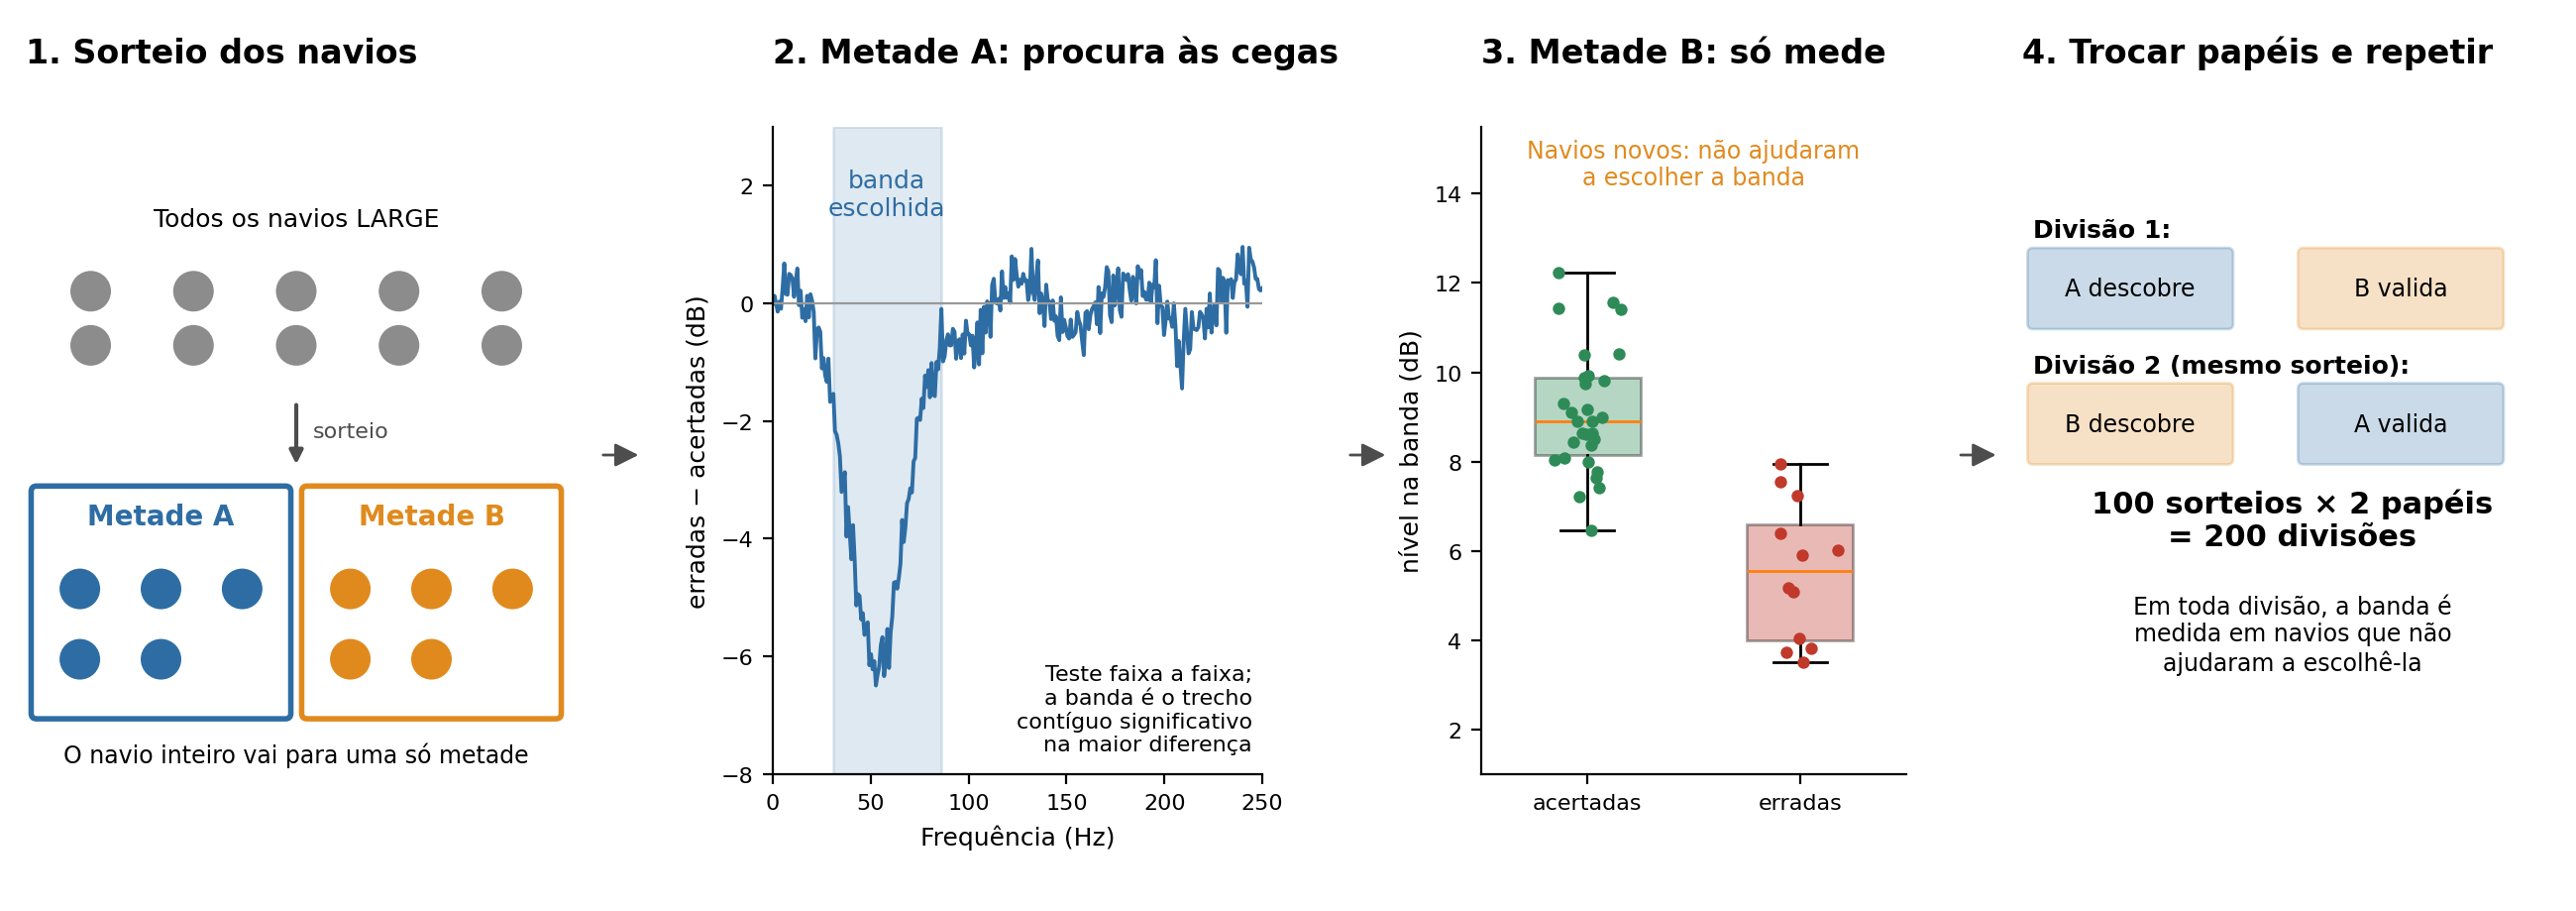
\includegraphics[width=0.93\textwidth]{validacao_metades_esquema.png}

    {\tiny Esquema ilustrativo (dados sintéticos).\par}
    \vspace{0.05cm}
    \begin{block}{\small Por que fazer isso}
        \scriptsize
        Achei a banda olhando todos os navios em 1.024 faixas, e alguma faixa sempre parece diferente por acaso. Por isso escolho a banda numa metade dos navios, às cegas, e meço o efeito na outra. Com 100 sorteios e as metades trocando de papel, são \textbf{200 divisões}.
    \end{block}
\end{frame}

\begin{frame}{Validação em Metades de Navios: Resultado}
    \centering
    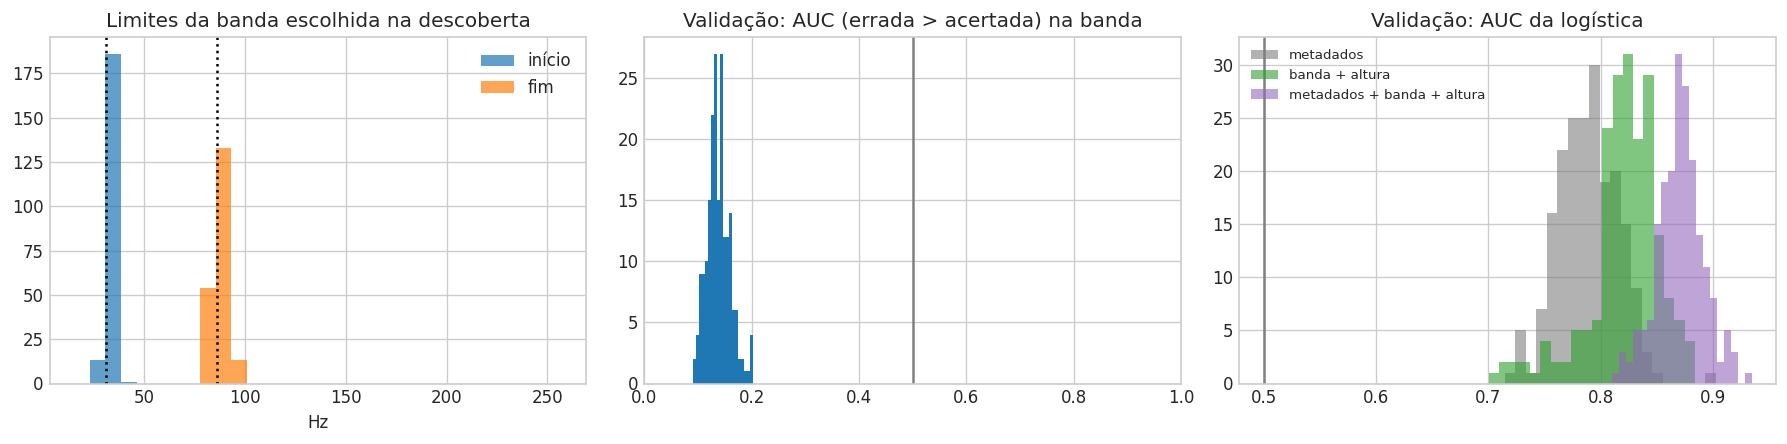
\includegraphics[width=0.95\textwidth]{lofar_large_validacao.png}

    {\tiny 100 sorteios $\times$ 2 papéis = 200 divisões.\par}
    \vspace{0.05cm}
    \begin{alertblock}{\small O achado se replica em navios novos}
        \scriptsize
        \begin{itemize}
            \setlength{\itemsep}{0pt}
            \item Nas 200 divisões, a procura às cegas encontrou uma banda; o intervalo mais frequente foi 31,2--85,9 Hz (122 vezes).
            \item Medida na outra metade, a diferença se confirmou: AUC mediana \textbf{0,14} (5--95\%: 0,10--0,17), p $<$ 0,05 em todas as divisões.
            \item Logística treinada numa metade: banda + altura prevê o erro com AUC \textbf{0,82}; metadados 0,79; tudo junto 0,87.
        \end{itemize}
    \end{alertblock}
\end{frame}

\begin{frame}{A Banda Depende da Gravação, Não do Navio}
    \footnotesize
    \begin{columns}[t]
        \column{0.52\textwidth}
        \begin{block}{\small 17 navios com gravações acertadas e erradas}\setlength{\tabcolsep}{3pt}
            \scriptsize
            \centering
            \begin{tabular}{lccc}
            \toprule
             & Acertadas & Erradas & Teste do sinal \\
            \midrule
            Banda (fração) & \textbf{0,81} & \textbf{0,24} & 12 $\times$ 2, \textbf{p = 0,013} \\
            Altura do pico & 11,7 dB & 9,6 dB & 11 $\times$ 6, p = 0,33 \\
            Vento & 4,8 m/s & 5,4 m/s & 7 $\times$ 8, p = 1,0 \\
            Estado do mar & 2,5 & 2,8 & 6 $\times$ 7, p = 1,0 \\
            \bottomrule
            \end{tabular}
        \end{block}
        \column{0.46\textwidth}
        \begin{block}{\small Quanto do erro cada fator explica}
            \scriptsize
            \centering
            Logística, CV agrupada por navio:

            \vspace{0.05cm}
            \begin{tabular}{lc}
            \toprule
            Atributos & AUC \\
            \midrule
            Só subconjunto & 0,72 \\
            Metadados (tipo, tamanho, vento...) & 0,80 \\
            Só a banda grave & \textbf{0,82} \\
            Banda + metadados & \textbf{0,88} \\
            \bottomrule
            \end{tabular}
        \end{block}
    \end{columns}
    \vspace{0.1cm}
    \begin{alertblock}{Leitura}
        \scriptsize
        No mesmo navio, a banda aparece nas gravações acertadas e falta nas erradas, sem diferença de vento ou mar. Ela não é uma assinatura fixa do navio: minha hipótese é que dependa do \textbf{regime de operação, da distância exata ou da propagação}. O IARA não registra velocidade nem a distância ao longo da gravação, só a faixa de distância do subconjunto e o instante do CPA.
    \end{alertblock}
\end{frame}

\begin{frame}{Banda Larga ou Raias? Faixas de 1 Hz (\texttt{lofar1hz})}
    \centering
    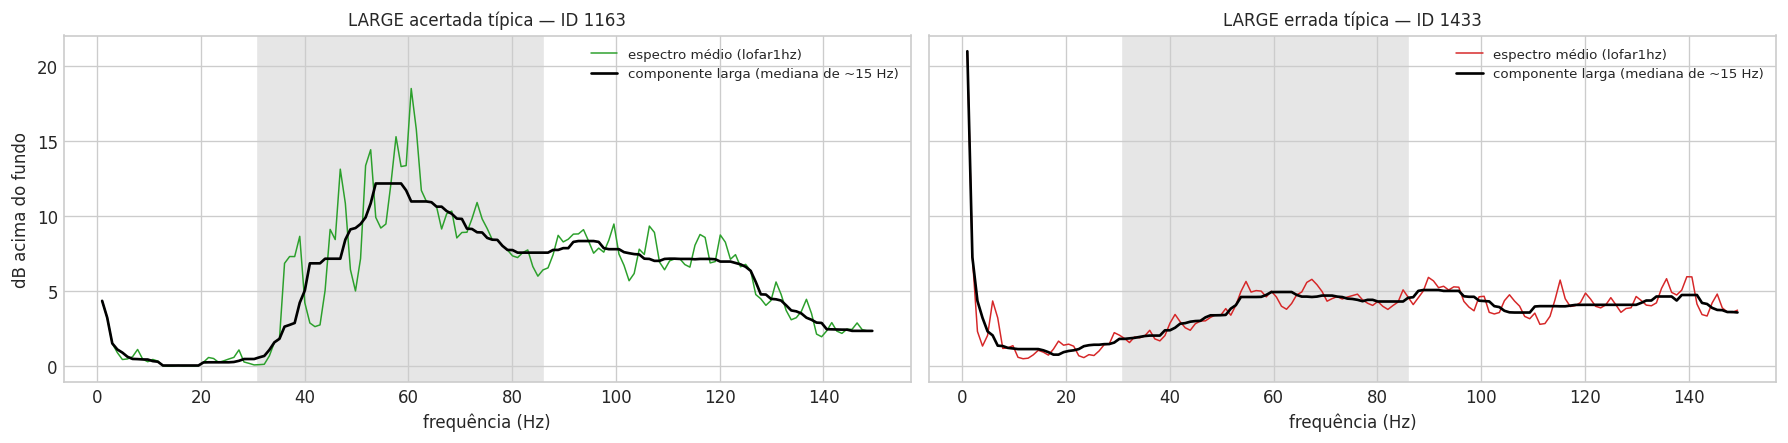
\includegraphics[width=0.95\textwidth]{lofar1hz_decomposicao.png}

    {\tiny Componente larga = mediana móvel de $\sim$15 Hz; raias = máximos locais $\geq$ 3 dB acima dela, em 31--86 Hz (faixa cinza).\par}
    \vspace{0.05cm}
    \begin{columns}[t]
        \column{0.49\textwidth}
        \begin{block}{\small Acertadas $\times$ erradas (por navio)}
            \scriptsize
            \centering
            \begin{tabular}{lcc}
            \toprule
             & Medianas & AUC \\
            \midrule
            Componente larga & 8,5 $\times$ 3,8 dB & \textbf{0,12} \\
            Energia das raias & 0,40 $\times$ 0,47 & 0,53 \\
            Número de raias & 2 $\times$ 2 & 0,51 \\
            \bottomrule
            \end{tabular}
        \end{block}
        \column{0.49\textwidth}
        \begin{block}{\small Leitura}
            \scriptsize
            O que separa é a \textbf{componente larga}; as raias existem nos dois grupos. Testei filtros de 11--21 faixas e proeminência de 2--6 dB: o resultado é estável. Raias espaçadas de menos de $\sim$2 Hz ainda não seriam resolvidas.
        \end{block}
    \end{columns}
\end{frame}

%===========================================
% SEÇÃO 3: MEDIUM E SMALL
%===========================================
\section{MEDIUM e SMALL: Erros por Destino}

\begin{frame}
    \centering
    \huge MEDIUM e SMALL: Erros por Destino
\end{frame}

\begin{frame}{Fora da Amostra: a Banda das LARGE nas Outras Classes}
    \footnotesize
    {\scriptsize\textbf{Fixei a hipótese antes de olhar os dados:} as MEDIUM e SMALL previstas como LARGE têm a banda. Como os navios são outros, apenas \textbf{medi} a banda, sem escolhê-la.\par}
    \vspace{0.1cm}
    \begin{table}
    \centering
    \scriptsize
    \begin{tabular}{llccc}
    \toprule
    Classe & Subgrupo & Banda 31--86 Hz (mediana) & AUC vs. acertadas & Navios mistos (sinal) \\
    \midrule
    \multirow{2}{*}{MEDIUM} & errada$\to$LARGE & \textbf{7,0 dB} (acertadas 3,9) & \textbf{0,82}, p $<$ 0,001 & \textbf{9 de 9}, p = 0,004 \\
     & errada$\to$SMALL & 3,4 dB & 0,47, p = 0,69 & 8 de 13, p = 0,58 \\
    \midrule
    \multirow{3}{*}{SMALL} & errada$\to$LARGE & \textbf{7,8 dB} (acertadas 4,6) & \textbf{0,85}, p $<$ 0,001 & 9 de 11, p = 0,065 \\
     & errada$\to$MEDIUM & 4,0 dB & 0,47, p = 0,69 & --- \\
     & errada$\to$BACKGR. & 2,3 dB & 0,23, p = 0,006 & --- \\
    \bottomrule
    \end{tabular}
    \end{table}
    \vspace{0.05cm}
    \begin{alertblock}{Leitura}
        \scriptsize
        \textbf{Confirmada fora da amostra}: as gravações chamadas de LARGE têm a banda no nível das LARGE (mediana 7,2 dB), e no mesmo navio ela aparece na gravação chamada de LARGE. No \texttt{lofar1hz}, de novo é componente larga (AUC 0,87). Os erros MEDIUM$\to$SMALL e SMALL$\to$MEDIUM \textbf{não têm assinatura} no LOFAR.
    \end{alertblock}
\end{frame}

\begin{frame}{A Banda é Pista do Modelo, Mas Fraca de Tamanho Real}
    \footnotesize
    \begin{columns}[t]
        \column{0.56\textwidth}
        \begin{block}{\small \% dos folds em que a gravação é prevista LARGE}
            \scriptsize
            \centering
            \setlength{\tabcolsep}{4pt}
            \begin{tabular}{lccc}
            \toprule
            Modelo & SMALL & MEDIUM & LARGE \\
             & sem $\to$ com & sem $\to$ com & sem $\to$ com \\
            \midrule
            CNN LOFAR & 11 $\to$ 37 & 6 $\to$ 23 & 39 $\to$ 83 \\
            CNN MEL & 8 $\to$ 31 & 6 $\to$ 21 & 36 $\to$ 78 \\
            SVM LOFAR & 14 $\to$ 48 & 9 $\to$ 33 & 44 $\to$ 88 \\
            SVM MEL & 9 $\to$ 30 & 8 $\to$ 21 & 39 $\to$ 80 \\
            RF LOFAR & 13 $\to$ 54 & 5 $\to$ 33 & 35 $\to$ 91 \\
            \bottomrule
            \end{tabular}

            \vspace{0.05cm}
            {\tiny ``com'' = pico grave em 31--86 Hz.\par}
        \end{block}
        \column{0.42\textwidth}
        \begin{block}{\small Quem tem a banda}
            \scriptsize
            \centering
            \begin{tabular}{lc}
            \toprule
            LARGE & 72\% \\
            SMALL & 43\% \\
            MEDIUM & 35\% \\
            \midrule
            Das gravações com banda, LARGE & 55\% \\
            \bottomrule
            \end{tabular}
        \end{block}
    \end{columns}
    \vspace{0.1cm}
    \begin{alertblock}{Leitura}
        \scriptsize
        Em todas as classes e modelos (inclusive MEL), ter a banda \textbf{aumenta a chance} de ser chamado de LARGE. \textbf{Não é uma regra}: a maioria das SMALL e MEDIUM com a banda não é chamada de LARGE. Mas, como a banda separa mal as classes reais, parte dos erros vem dela: falta em LARGE (que viram SMALL/MEDIUM) e aparece em SMALL/MEDIUM (que viram LARGE).
    \end{alertblock}
\end{frame}

\begin{frame}{MEDIUM: o Espectro por Destino do Erro}
    \centering
    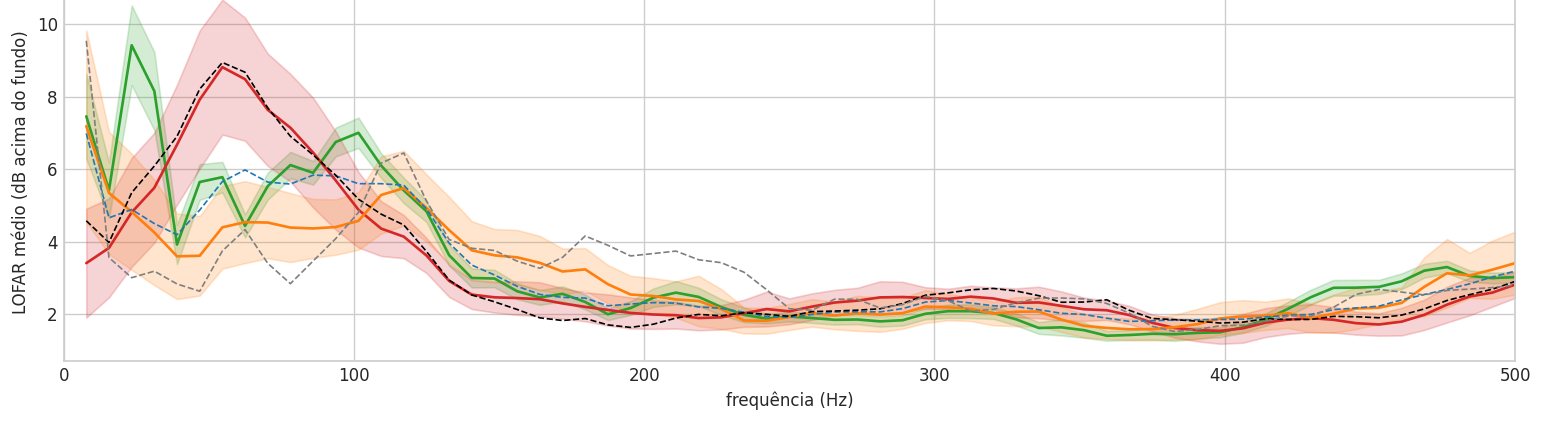
\includegraphics[width=0.92\textwidth]{lofar_medium_espectro_zoom.png}

    {\tiny Espectro LOFAR médio, 0--500 Hz. \textcolor{greenwin}{Verde}: MEDIUM acertadas (193); \textcolor{red}{vermelho}: erradas$\to$LARGE (35); \textcolor{orange}{laranja}: erradas$\to$SMALL (36). Tracejadas: SMALL (azul), LARGE (preto), BACKGROUND (cinza).\par}
    \vspace{0.05cm}
    \begin{alertblock}{Leitura}
        \scriptsize
        As erradas$\to$LARGE seguem a curva das LARGE (0,28 dB RMS). As acertadas \textbf{não diferem de SMALL em nenhuma das 1.024 faixas} (contra LARGE: 500 faixas). Os erros$\to$SMALL também não diferem das acertadas em nenhuma faixa.
    \end{alertblock}
\end{frame}

\begin{frame}{MEDIUM Acertadas: Padrão ou Navios Conhecidos?}
    \footnotesize
    \begin{columns}[t]
        \column{0.55\textwidth}
        \begin{block}{\small Acerto da CNN LOFAR pelo nº de gravações do navio}
            \scriptsize
            \centering
            \begin{tabular}{lccc}
            \toprule
            Gravações do navio & MEDIUM & SMALL & LARGE \\
            \midrule
            1 & \calo{25\%} & 20\% & 63\% \\
            2--3 & 32\% & 29\% & 56\% \\
            4--10 & 31\% & 26\% & 46\% \\
            mais de 10 & \cahi{64\%} & 26\% & 69\% \\
            \bottomrule
            \end{tabular}

            \vspace{0.05cm}
            {\tiny \% de gravações acertadas em todos os folds.\par}
        \end{block}
        \column{0.43\textwidth}
        \begin{block}{\small Concentração}
            \scriptsize
            \begin{itemize}
                \setlength{\itemsep}{1pt}
                \item 138 das 193 MEDIUM acertadas (\textbf{72\%}) vêm de 7 navios gravados mais de 10 vezes.
                \item 2 Motor Hoppers irmãos (HANG BO 2002/2003) somam \textbf{37\%} das gravações MEDIUM.
                \item O split do artigo é \textbf{por gravação}: em todo fold, $\sim$25--35 gravações do HANG BO 2003 estão no teste e o resto no treino.
            \end{itemize}
        \end{block}
    \end{columns}
    \vspace{0.1cm}
    \begin{alertblock}{Leitura}
        \scriptsize
        O acerto em MEDIUM vem mais de \textbf{reconhecer navios já vistos} do que de um padrão de frequência. Em LARGE, a curva é plana: lá a banda generaliza para navios novos. Em SMALL, o acerto é baixo mesmo para navios conhecidos.
    \end{alertblock}
\end{frame}

\begin{frame}{Com Split por Navio, MEDIUM Desaba em Todos os Modelos}
    \footnotesize
    \begin{columns}[t]
        \column{0.55\textwidth}
        \begin{block}{\small Recall de MEDIUM: split por gravação $\to$ por navio (NB29)}
            \scriptsize
            \centering
            \begin{tabular}{lcc}
            \toprule
            Modelo & Recall MEDIUM (\%) & Acc. bal. \\
            \midrule
            SVM MEL & 52,5 $\to$ \calo{31,4} & $-8{,}6$ \\
            SVM LOFAR & 55,0 $\to$ \calo{32,9} & $-5{,}4$ \\
            MLP MEL & 68,5 $\to$ \calo{41,0} & $-8{,}5$ \\
            MLP LOFAR & 65,9 $\to$ \calo{34,5} & $-9{,}6$ \\
            RF MEL & 51,9 $\to$ \calo{29,2} & $-9{,}5$ \\
            RF LOFAR & 40,0 $\to$ \calo{23,1} & $-8{,}4$ \\
            BiGRU LOFAR & 50,5 $\to$ \calo{27,6} & $-9{,}2$ \\
            \bottomrule
            \end{tabular}

            \vspace{0.05cm}
            {\tiny Mesmo código e sementes; só muda a regra de divisão. Queda média: MEDIUM $-23$ p.p., SMALL $-5{,}5$, LARGE $-3{,}4$, BACKGROUND $-0{,}2$.\par}
        \end{block}
        \column{0.43\textwidth}
        \begin{block}{\small Motor Hoppers irmãos (split por navio)}
            \scriptsize
            \centering
            Reconhecidos como MEDIUM:

            \vspace{0.05cm}
            \begin{tabular}{lcc}
            \toprule
            Modelo & Irmão no treino & Nenhum \\
            \midrule
            MLP LOFAR & 77\% & 8\% \\
            MLP MEL & 71\% & 13\% \\
            SVM MEL & 64\% & 2\% \\
            BiGRU LOFAR & 57\% & 7\% \\
            RF LOFAR & 54\% & 0\% \\
            \bottomrule
            \end{tabular}
        \end{block}
    \end{columns}
    \vspace{0.1cm}
    \begin{alertblock}{Leitura}
        \scriptsize
        Em navios novos, MEDIUM fica entre 23\% e 41\% (acaso com 4 classes: 25\%). Os modelos aprendem \textbf{identidade do navio ou da série} (``este é um HANG BO''), não \textbf{classe de tamanho}. Não é falta de capacidade do modelo: é o dado.
    \end{alertblock}
\end{frame}

%===========================================
% SEÇÃO 4: DEMON
%===========================================
\section{DEMON: Picos de Modulação}

\begin{frame}
    \centering
    \huge DEMON: Picos de Modulação
\end{frame}

\begin{frame}{DEMON: a Fundamental Cai com o Comprimento}
    \centering
    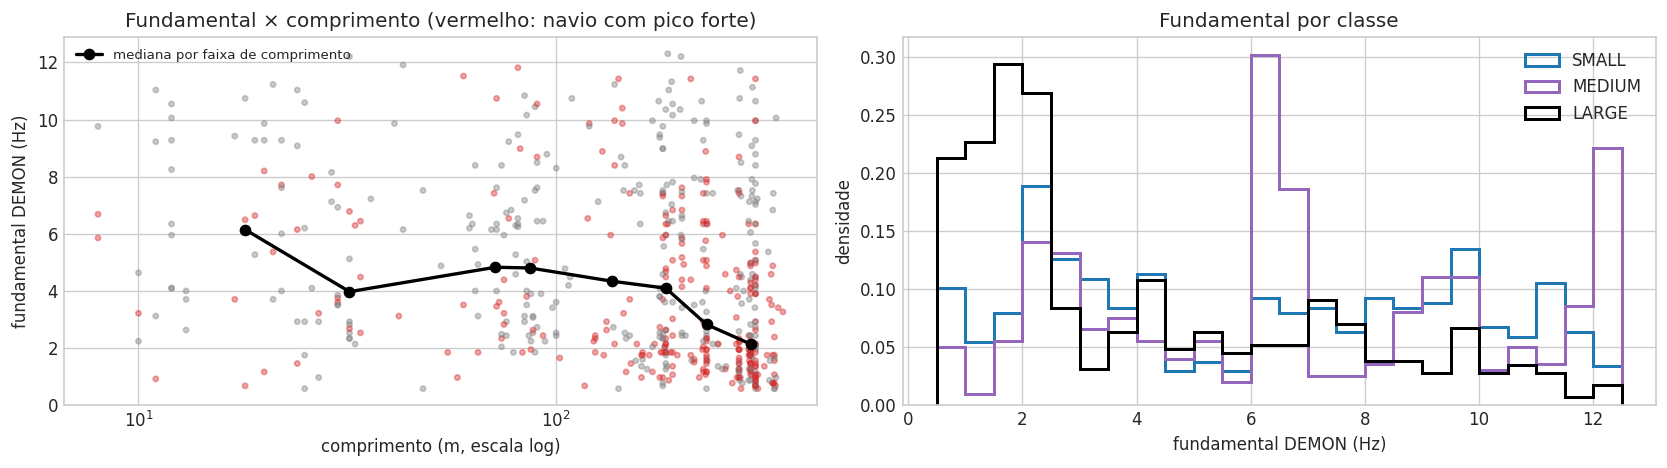
\includegraphics[width=0.92\textwidth]{demon_fundamental.png}

    {\tiny DEMON do projeto (1--2 kHz, 0,39--25 Hz), em dB acima do fundo TPSW. Fundamental = frequência cujos múltiplos (f, 2f, 3f, 4f) somam mais energia. Modelo de referência: BiGRU DEMON (SP 55,5).\par}
    \vspace{0.05cm}
    \begin{alertblock}{Leitura}
        \scriptsize
        \begin{itemize}
            \setlength{\itemsep}{0pt}
            \item Fundamental mediana: SMALL 6,3 Hz, MEDIUM 6,4 Hz, \textbf{LARGE 2,4 Hz}. Pico forte ($\geq$ 10 dB): 28\%, 24\% e \textbf{49\%}. \textbf{SMALL e MEDIUM são iguais}, como no LOFAR.
            \item $\rho = -0{,}31$ com o comprimento (586 navios), no sentido físico esperado, mas \textbf{não gradual}: fica em 4--5 Hz de 25 a 200 m e só cai acima de 200 m. O pico de MEDIUM em 6--7 Hz são os Motor Hoppers.
        \end{itemize}
    \end{alertblock}
\end{frame}

\begin{frame}{DEMON: Acertadas $\times$ Erradas e o Pico Forte}
    \footnotesize
    \begin{columns}[t]
        \column{0.53\textwidth}
        \begin{block}{\small Pico dominante, por destino do erro}
            \scriptsize
            \centering
            \setlength{\tabcolsep}{3pt}
            \begin{tabular}{llcc}
            \toprule
            Classe & Subgrupo & Fundamental & Pico forte \\
            \midrule
            \multirow{2}{*}{LARGE} & acertadas & 2,1 Hz & 66\% \\
             & errada$\to$SMALL & 5,6 Hz & 21\% \\
            \midrule
            \multirow{2}{*}{MEDIUM} & acertadas & 6,7 Hz & 25\% \\
             & errada$\to$LARGE & \textbf{3,7 Hz} & \textbf{48\%} \\
            \midrule
            \multirow{2}{*}{SMALL} & acertadas & 7,1 Hz & 16\% \\
             & errada$\to$LARGE & 3,9 Hz & \textbf{53\%} \\
            \bottomrule
            \end{tabular}
        \end{block}
        \column{0.45\textwidth}
        \begin{block}{\small O pico forte como pista de LARGE}
            \scriptsize
            Previsto LARGE (BiGRU), sem $\to$ com pico forte:

            \vspace{0.05cm}
            \centering
            \begin{tabular}{lc}
            \toprule
            SMALL & 17 $\to$ 42\% \\
            MEDIUM & 9 $\to$ 23\% \\
            LARGE & 48 $\to$ 78\% \\
            \bottomrule
            \end{tabular}

            \vspace{0.05cm}
            \raggedright
            Mesmo resultado com limiares de 6 a 15 dB.
        \end{block}
    \end{columns}
    \vspace{0.1cm}
    \begin{alertblock}{Leitura}
        \scriptsize
        O DEMON repete o LOFAR: um \textbf{pico forte e grave} é a pista de LARGE, também fraca de tamanho real. As duas pistas andam juntas (pico forte em 56\% das LARGE com a banda LOFAR, 31\% sem), talvez o mesmo regime da hélice (não verifiquei). Ressalva: modelos DEMON são mais fracos, rótulos mais ruidosos.
    \end{alertblock}
\end{frame}

%===========================================
% SEÇÃO 5: OSS × TUG
%===========================================
\section{Offshore Supply Ships $\times$ Rebocadores}

\begin{frame}
    \centering
    \huge Offshore Supply Ships $\times$ Rebocadores
\end{frame}

\begin{frame}{Por Que Olhei Esse Par}
    \footnotesize
    \begin{columns}[t]
        \column{0.6\textwidth}
        \begin{block}{\small Recall de MEDIUM por tipo de navio}
            \scriptsize
            \centering
            \setlength{\tabcolsep}{2pt}
            \begin{tabular}{lcccc}
            \toprule
            Tipo & Grav. & Navios & CNN LOFAR & MLP LOFAR \\
             & & & (gravação) & (grav. $\to$ navio) \\
            \midrule
            Motor Hopper & 147 & 3 & 88\% & 89 $\to$ \calo{36\%} \\
            Offshore Supply & 139 & 46 & 54\% & 51 $\to$ \calo{32\%} \\
            Supply Vessel & 33 & 7 & 48\% & 39 $\to$ 19\% \\
            Anchor Handling & 32 & 6 & 41\% & 65 $\to$ 34\% \\
            \bottomrule
            \end{tabular}
        \end{block}
        \column{0.38\textwidth}
        \begin{block}{\small LOFAR médio, q $<$ 0,05}
            \scriptsize
            \centering
            \begin{tabular}{lc}
            \toprule
            OSS $\times$ Tug (SMALL) & \calo{\textbf{0}} \\
            OSS $\times$ Fishing (SMALL) & \calo{\textbf{0}} \\
            OSS $\times$ Pilot (SMALL) & 527 \\
            OSS $\times$ LARGE & 458 \\
            \bottomrule
            \end{tabular}

            \vspace{0.05cm}
            {\tiny 46 OSS (53--93 m) e 34 rebocadores (18--34 m).\par}
        \end{block}
    \end{columns}
    \vspace{0.1cm}
    \begin{alertblock}{Pergunta}
        \scriptsize
        O OSS é o tipo MEDIUM com mais navios distintos (46): o melhor teste de generalização. Mesmo assim fica perto do acaso em navios novos, e no LOFAR é \textbf{igual a rebocadores}. Alguma representação que os modelos \textbf{não} usam separa os dois?
    \end{alertblock}
\end{frame}

\begin{frame}{Sete Representações, Nenhuma Separação Espectral}
    \footnotesize
    \begin{table}
    \centering
    \scriptsize
    \begin{tabular}{lp{7.4cm}c}
    \toprule
    \textbf{Representação} & \textbf{O que comparei (OSS $\times$ Tug, por navio)} & \textbf{Separa?} \\
    \midrule
    LOFAR (pipeline) & 1.024 faixas do espectro médio & \calo{0 faixas} \\
    \texttt{lofar1hz} & Posição das raias persistentes (melhor: 78 Hz, q = 0,22) & \calo{0 faixas} \\
    \texttt{psd24k} & Forma do espectro 20 Hz--23 kHz (3.922 faixas) & \calo{0 faixas} \\
    DEMON (5 bandas) & Espectro e pico dominante em 0,5--16 kHz & \calo{$\leq$ 1 faixa} \\
    MEL (entrada L2) & 256 bandas, dentro de cada subconjunto & \calo{0 faixas} \\
    HHT 1D e 2D & Espectro marginal e médio, dentro de cada subconjunto & \calo{0 faixas} \\
    \midrule
    Nível absoluto & Nível médio em 1--8 kHz (\texttt{psd24k}) & \camd{AUC 0,77} \\
    HHT 2D ``intermitência'' & CV da energia em passos de 80 ms, 100--200 Hz & \camd{AUC $\sim$0,3} \\
    \bottomrule
    \end{tabular}
    \end{table}
    \vspace{0.05cm}
    \begin{alertblock}{Leitura}
        \scriptsize
        Nenhuma representação espectral separa os OSS dos rebocadores dentro de um subconjunto, \textbf{nem a alta frequência até 24 kHz}. Analiso as duas exceções (amarelo) nos próximos slides: uma é instrumental, a outra é energia relativa.
    \end{alertblock}
\end{frame}

\begin{frame}{Forma do Espectro até 24 kHz e o Nível}
    \centering
    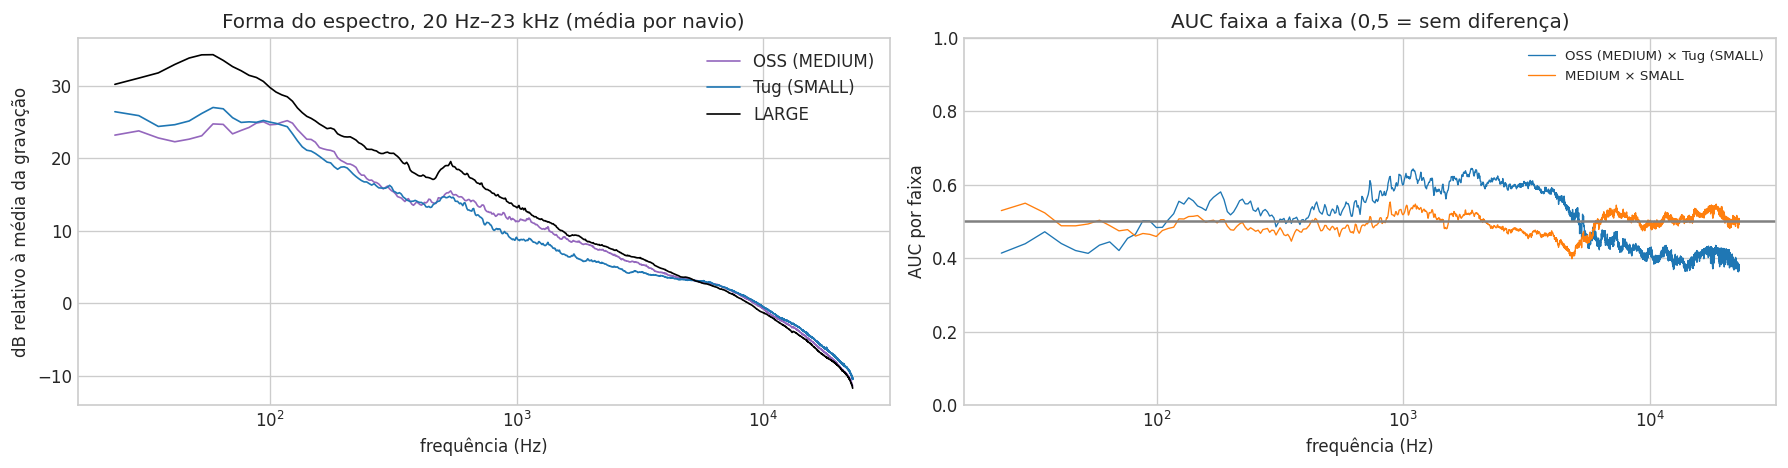
\includegraphics[width=0.92\textwidth]{psd24k_oss_tug.png}
    \vspace{0.05cm}
    \begin{columns}[t]
        \column{0.49\textwidth}
        \begin{block}{\small Nível (por navio)}
            \scriptsize
            \centering
            \setlength{\tabcolsep}{3pt}
            \begin{tabular}{lcc}
            \toprule
             & AUC OSS $\times$ Tug & Ganho? \\
            \midrule
            Nível médio & 0,77 & depende \\
            Trecho mais silencioso & 0,74 & depende \\
            Faixa dinâmica & 0,59 (p = 0,17) & \textbf{não dep.} \\
            \bottomrule
            \end{tabular}
        \end{block}
        \column{0.49\textwidth}
        \begin{block}{\small O nível é instrumental}
            \scriptsize
            A diferença aparece igual no \textbf{trecho mais silencioso} (equipamento e ruído do local) e some na faixa dinâmica. O IARA é 16 bits sem calibração (hidrofones de $-200$ a $-150$ dB re 1 V/µPa) e não diz qual hidrofone gravou cada arquivo.
        \end{block}
    \end{columns}
\end{frame}

\begin{frame}{HHT: ``Intermitência'' é Energia Relativa}\vspace{-0.25cm}
    \footnotesize
    \begin{columns}[t]
        \column{0.49\textwidth}
        \begin{block}{\small O que observei}
            \scriptsize
            \begin{itemize}
                \setlength{\itemsep}{1pt}
                \item CV no tempo (HHT 2D): 17 de 80 faixas diferem (100--200 e 730--830 Hz), maior nos rebocadores.
                \item Mesmo sentido nos 4 subconjuntos e em 95\% das metades de navios; p $<$ 0,05 em só 46\%.
            \end{itemize}
        \end{block}
        \column{0.49\textwidth}
        \begin{block}{\small O que ela mede de fato}
            \scriptsize
            \begin{itemize}
                \setlength{\itemsep}{1pt}
                \item Cada janela é normalizada pelo pico: faixa fraca $\Rightarrow$ média pequena $\Rightarrow$ CV grande.
                \item $\rho = -0{,}92$ com a energia relativa; descontada ela, sobra AUC 0,37 (p = 0,045).
            \end{itemize}
        \end{block}
    \end{columns}
    \vspace{0.1cm}
    \begin{block}{\small Frequência dominante: uma tendência fraca}
        \scriptsize
        \centering
        \begin{tabular}{lccc}
        \toprule
         & OSS & Tug & \\
        \midrule
        Pico dominante do LOFAR em 86--150 Hz & 21 de 46 navios & 7 de 34 & Fisher p = 0,03 \\
        Pico dominante do HHT 2D $\geq$ 86 Hz & 17 de 46 & 6 de 34 & p = 0,08 \\
        \bottomrule
        \end{tabular}
    \end{block}
    \vspace{0.05cm}
    \begin{alertblock}{Leitura}
        \scriptsize
        Os OSS têm \textbf{relativamente mais energia em $\sim$100--200 Hz}: diferença de balanço espectral, fraca e exploratória (encontrei-a depois de testar muitas representações).
    \end{alertblock}
\end{frame}

\begin{frame}{Teste Prático: Classificador com Split por Navio}
    \centering
    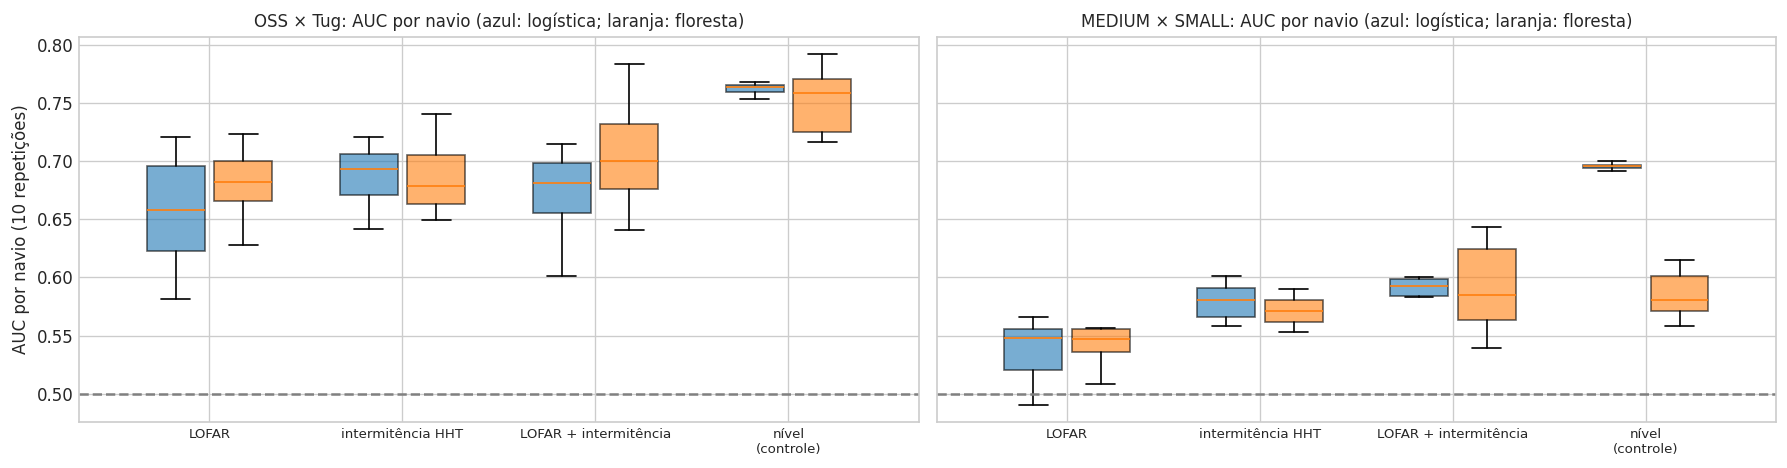
\includegraphics[width=0.95\textwidth]{classificador.png}

    {\tiny Treinei logística (PCA no fold) e floresta; 5 folds agrupados por navio $\times$ 10 sementes; cada navio pesa 1 no treino; AUC por navio.\par}
    \vspace{0.05cm}
    \begin{alertblock}{Leitura}
        \scriptsize
        \begin{itemize}
            \setlength{\itemsep}{0pt}
            \item \textbf{MEDIUM $\times$ SMALL}: LOFAR sozinho AUC 0,54--0,55; com a intermitência, 0,59 (ganho em 100\% das repetições, mas \textbf{perto do acaso}).
            \item \textbf{OSS $\times$ Tug}: $\sim$0,67--0,70, mas o \textbf{controle de nível}, sabidamente instrumental, dá 0,76. Uma AUC de $\sim$0,7 aqui não prova que o modelo aprendeu o som do navio.
        \end{itemize}
    \end{alertblock}
\end{frame}

\begin{frame}{Ouvindo os Pares}
    \begin{columns}[c]
        \column{0.5\textwidth}
        \centering
        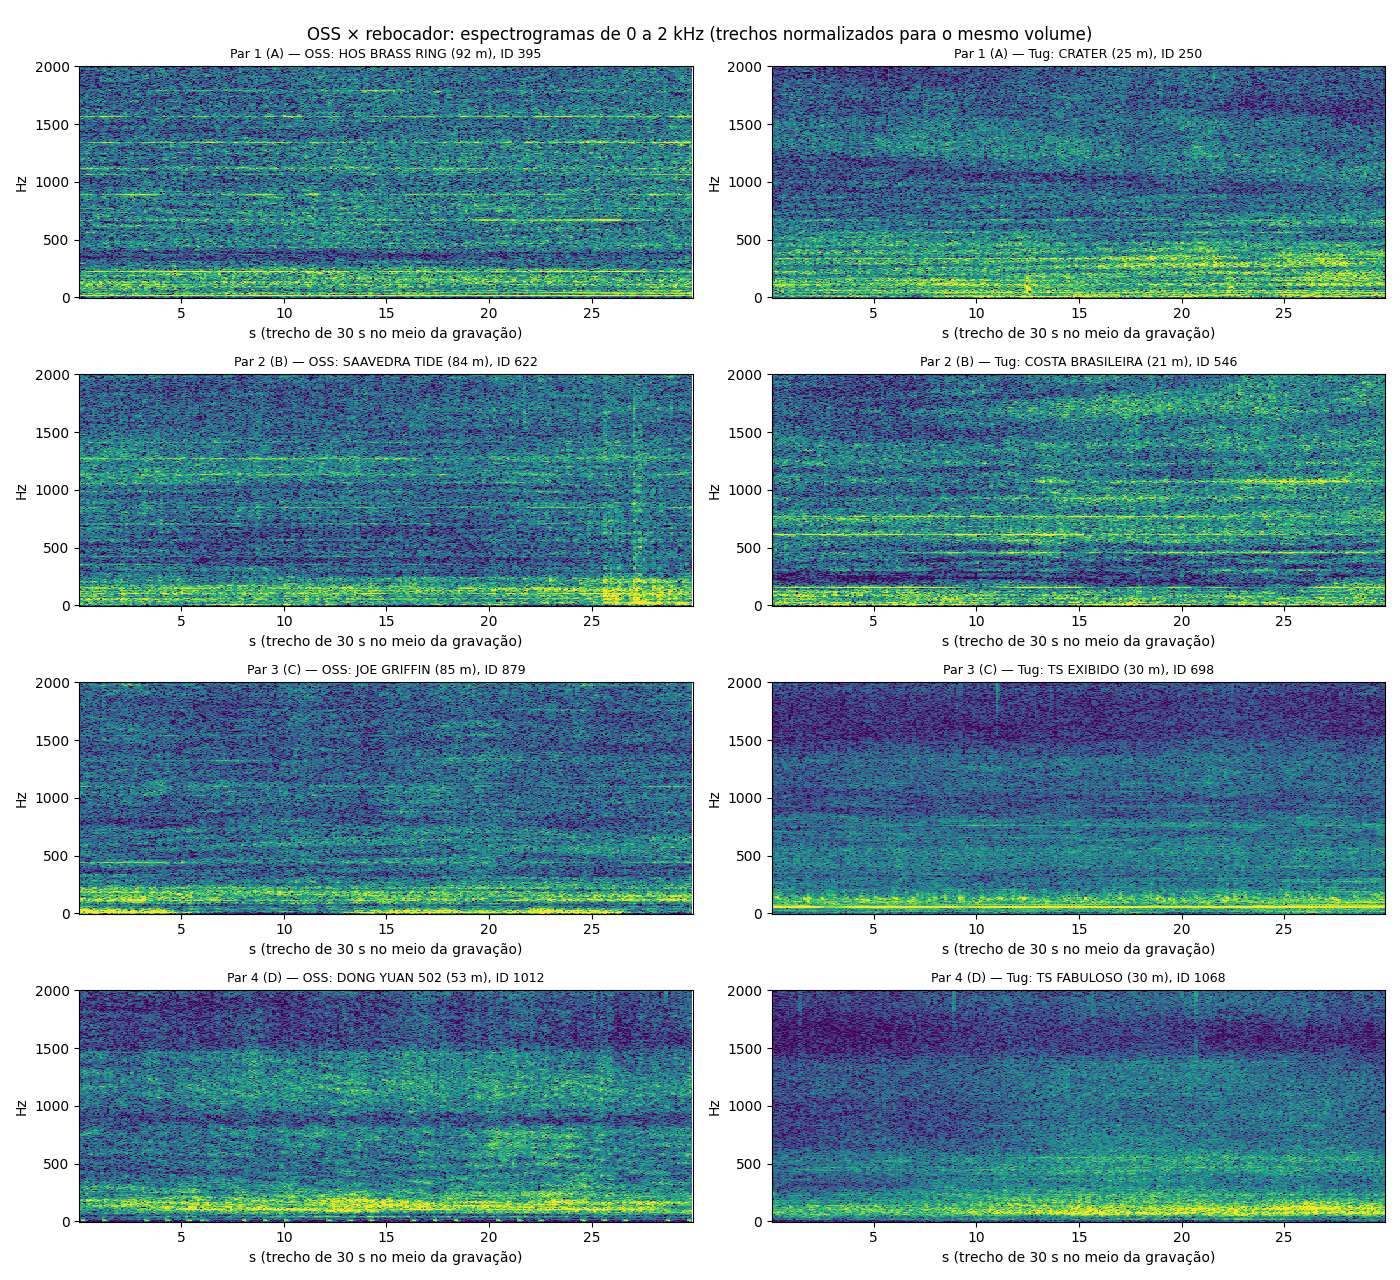
\includegraphics[width=\textwidth]{pares_oss_tug.png}
        \column{0.48\textwidth}
        \begin{block}{\small Separei 4 pares, um por subconjunto}
            \scriptsize
            \begin{tabular}{cll}
            \toprule
            & OSS (MEDIUM) & Tug (SMALL) \\
            \midrule
            A & HOS Brass Ring & Crater \\
            B & Saavedra Tide & Costa Brasileira \\
            C & Joe Griffin & TS Exibido \\
            D & Dong Yuan 502 & TS Fabuloso \\
            \bottomrule
            \end{tabular}

            \vspace{0.1cm}
            Trechos de 30 s no meio da gravação, normalizados para o \textbf{mesmo volume} (o nível absoluto é instrumental). Arquivos em \texttt{data/escuta\_oss\_tug/}.
        \end{block}
        \begin{alertblock}{Leitura}
            \scriptsize
            Nos espectrogramas de 0--2 kHz, não vejo nada que separe os tipos. Nos espectros médios, a distância RMS entre OSS e Tug (0,51 dB) é menor que a variação dentro de cada tipo ($\sim$1,2 dB).
        \end{alertblock}
    \end{columns}
\end{frame}

%===========================================
% SEÇÃO 6: CONCLUSÕES
%===========================================
\section{Conclusões}

\begin{frame}
    \centering
    \huge Conclusões
\end{frame}

\begin{frame}{Conclusões}
    \footnotesize
    \begin{enumerate}
        \setlength{\itemsep}{3pt}
        \item \textbf{LARGE tem assinatura acústica} em várias representações independentes: banda larga em 31--86 Hz (LOFAR), modulação forte e grave (DEMON) e maior faixa dinâmica na passagem (\texttt{psd24k}, AUC 0,69 contra MEDIUM). Validada em navios novos.
        \item \textbf{Essa assinatura é a principal pista dos modelos para LARGE}, em todas as famílias e entradas, mas é fraca de tamanho real: depende da gravação (no mesmo navio, aparece numa e falta noutra) e ocorre em $\sim$40\% das SMALL e MEDIUM. Explica boa parte dos erros envolvendo LARGE.
        \item \textbf{Não encontrei diferença acústica entre SMALL e MEDIUM} nestes dados: nem no LOFAR, MEL, DEMON, HHT, nem no espectro até 24 kHz. Um supply de 50--90 m soa como um rebocador de 20--35 m (propulsão parecida; hipótese física).
        \item \textbf{O recall de MEDIUM do split por gravação ($\sim$60\%) mede reconhecimento de navios repetidos}, sobretudo dos Motor Hoppers irmãos. Com split por navio, MEDIUM fica em 23--41\% em todos os modelos.
        \item \textbf{Concluo que o limite é do dado e do rótulo, não do modelo}: trocar SVM por CNN, ou LOFAR por MEL, não resolve, porque todos aprendem as mesmas pistas.
    \end{enumerate}
\end{frame}

\begin{frame}{Implicações e Próximos Passos}
    \footnotesize
    \begin{columns}[t]
        \column{0.49\textwidth}
        \begin{block}{\small Para a dissertação e o artigo}
            \scriptsize
            \begin{itemize}
                \setlength{\itemsep}{1pt}
                \item Pretendo relatar os resultados principais também com \textbf{split por navio}; o split por gravação superestima MEDIUM.
                \item Pretendo discutir que a fronteira SMALL/MEDIUM por comprimento quase não tem correlato acústico no IARA.
                \item Falta avaliar as CNNs do artigo com split por navio.
            \end{itemize}
        \end{block}
        \column{0.49\textwidth}
        \begin{block}{\small Experimentos que proponho}
            \scriptsize
            \begin{itemize}
                \setlength{\itemsep}{1pt}
                \item Retirar os Motor Hoppers e retreinar com split por navio ($\sim$40 min).
                \item Curva de aprendizado por nº de navios MEDIUM: falta dado ou falta informação?
                \item Formulações alternativas: juntar SMALL+MEDIUM, regressão do comprimento, ou classes por tipo de navio.
                \item HHT modificada (Tarefa 2b) para OSS $\times$ Tug.
            \end{itemize}
        \end{block}
    \end{columns}
    \vspace{0.1cm}
    \begin{alertblock}{O que destravaria a fronteira SMALL/MEDIUM}
        \scriptsize
        Metadados que o IARA não publica: \textbf{calibração e hidrofone} de cada gravação, \textbf{distância} ao navio e \textbf{velocidade (AIS)}. Com eles, o nível de fonte, a medida física mais direta de porte, passaria a ser utilizável. Proponho consultar os autores do dataset.
    \end{alertblock}
\end{frame}

\begin{frame}{Ressalvas}
    \footnotesize
    \begin{itemize}
        \setlength{\itemsep}{3pt}
        \item \textbf{``Não detectável'' não é ``não existe''}: 46 OSS e 34 rebocadores dão poder para diferenças moderadas, não pequenas.
        \item \textbf{Análises exploratórias}: testei muitas representações e faixas. Considero os achados positivos de OSS $\times$ Tug (frequência dominante, energia relativa) indícios, não resultados. A banda das LARGE, ao contrário, validei em metades de navios e fora da amostra.
        \item \textbf{Causa da banda}: regime de operação, distância e propagação são hipóteses minhas; o IARA não registra velocidade nem a distância ao longo da gravação. Registra a faixa de distância de cada subconjunto (até 250 m em A/B, 250--500 m em C/D) e, em A e C, o instante do CPA. A diferença da banda aparece dentro de cada subconjunto.
        \item \textbf{DEMON}: os modelos de referência são mais fracos (SP $\sim$55), então os rótulos de acerto e erro são mais ruidosos; o resultado mais sólido é a relação fundamental $\times$ comprimento, que não depende do modelo.
        \item \textbf{Efeito de borda do TPSW} abaixo de $\sim$150 Hz: afeta valores absolutos, não a comparação entre grupos.
    \end{itemize}
\end{frame}

%===========================================
% SLIDE FINAL
%===========================================
\begin{frame}
    \centering
    \Huge Obrigado!

    \vspace{0.8cm}
    \normalsize
    Evandro Rocha\\
    UFRJ / COPPE / PEE
\end{frame}

%===========================================
% APÊNDICE
%===========================================
\appendix

\begin{frame}{Apêndice: Exemplos de Espectrogramas LOFAR (LARGE)}
    \centering
    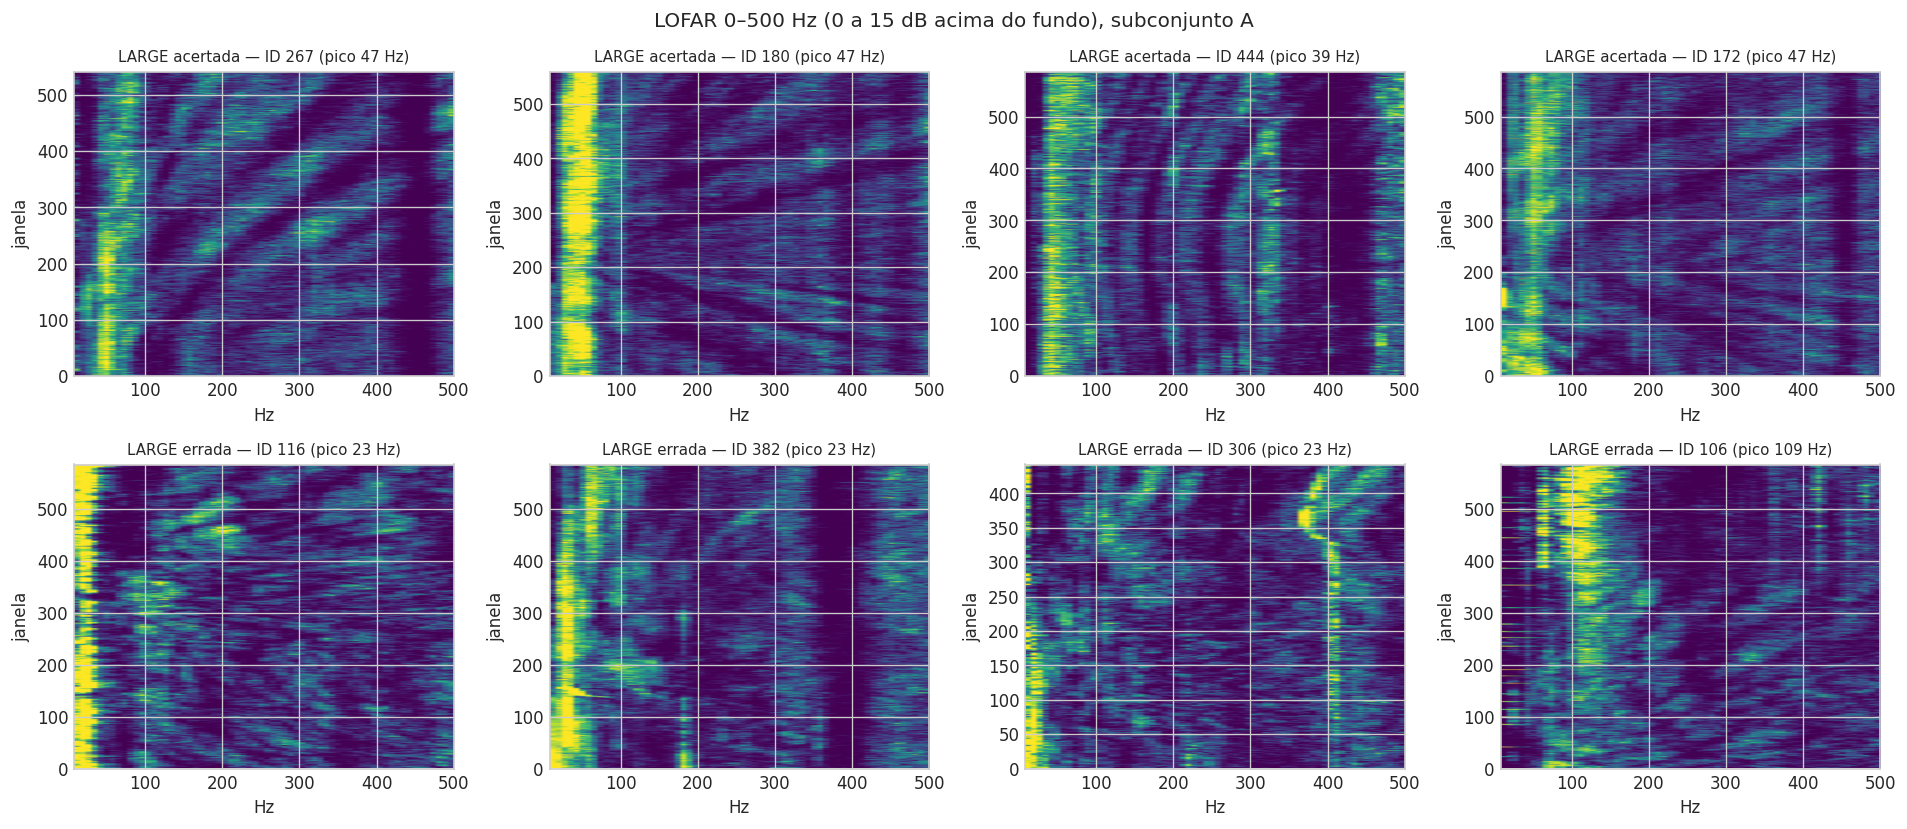
\includegraphics[width=0.95\textwidth]{lofar_large_exemplos.png}

    {\tiny Subconjunto A, 0--500 Hz, 0 a 15 dB acima do fundo. Linha de cima: acertadas (banda clara e estável em $\sim$30--80 Hz). Linha de baixo: erradas (energia abaixo de $\sim$30 Hz ou acima de $\sim$90 Hz).\par}
\end{frame}

\begin{frame}{Apêndice: Extração do LOFAR do Pipeline}
    \begin{columns}[c]
        \column{0.36\textwidth}
        \centering
        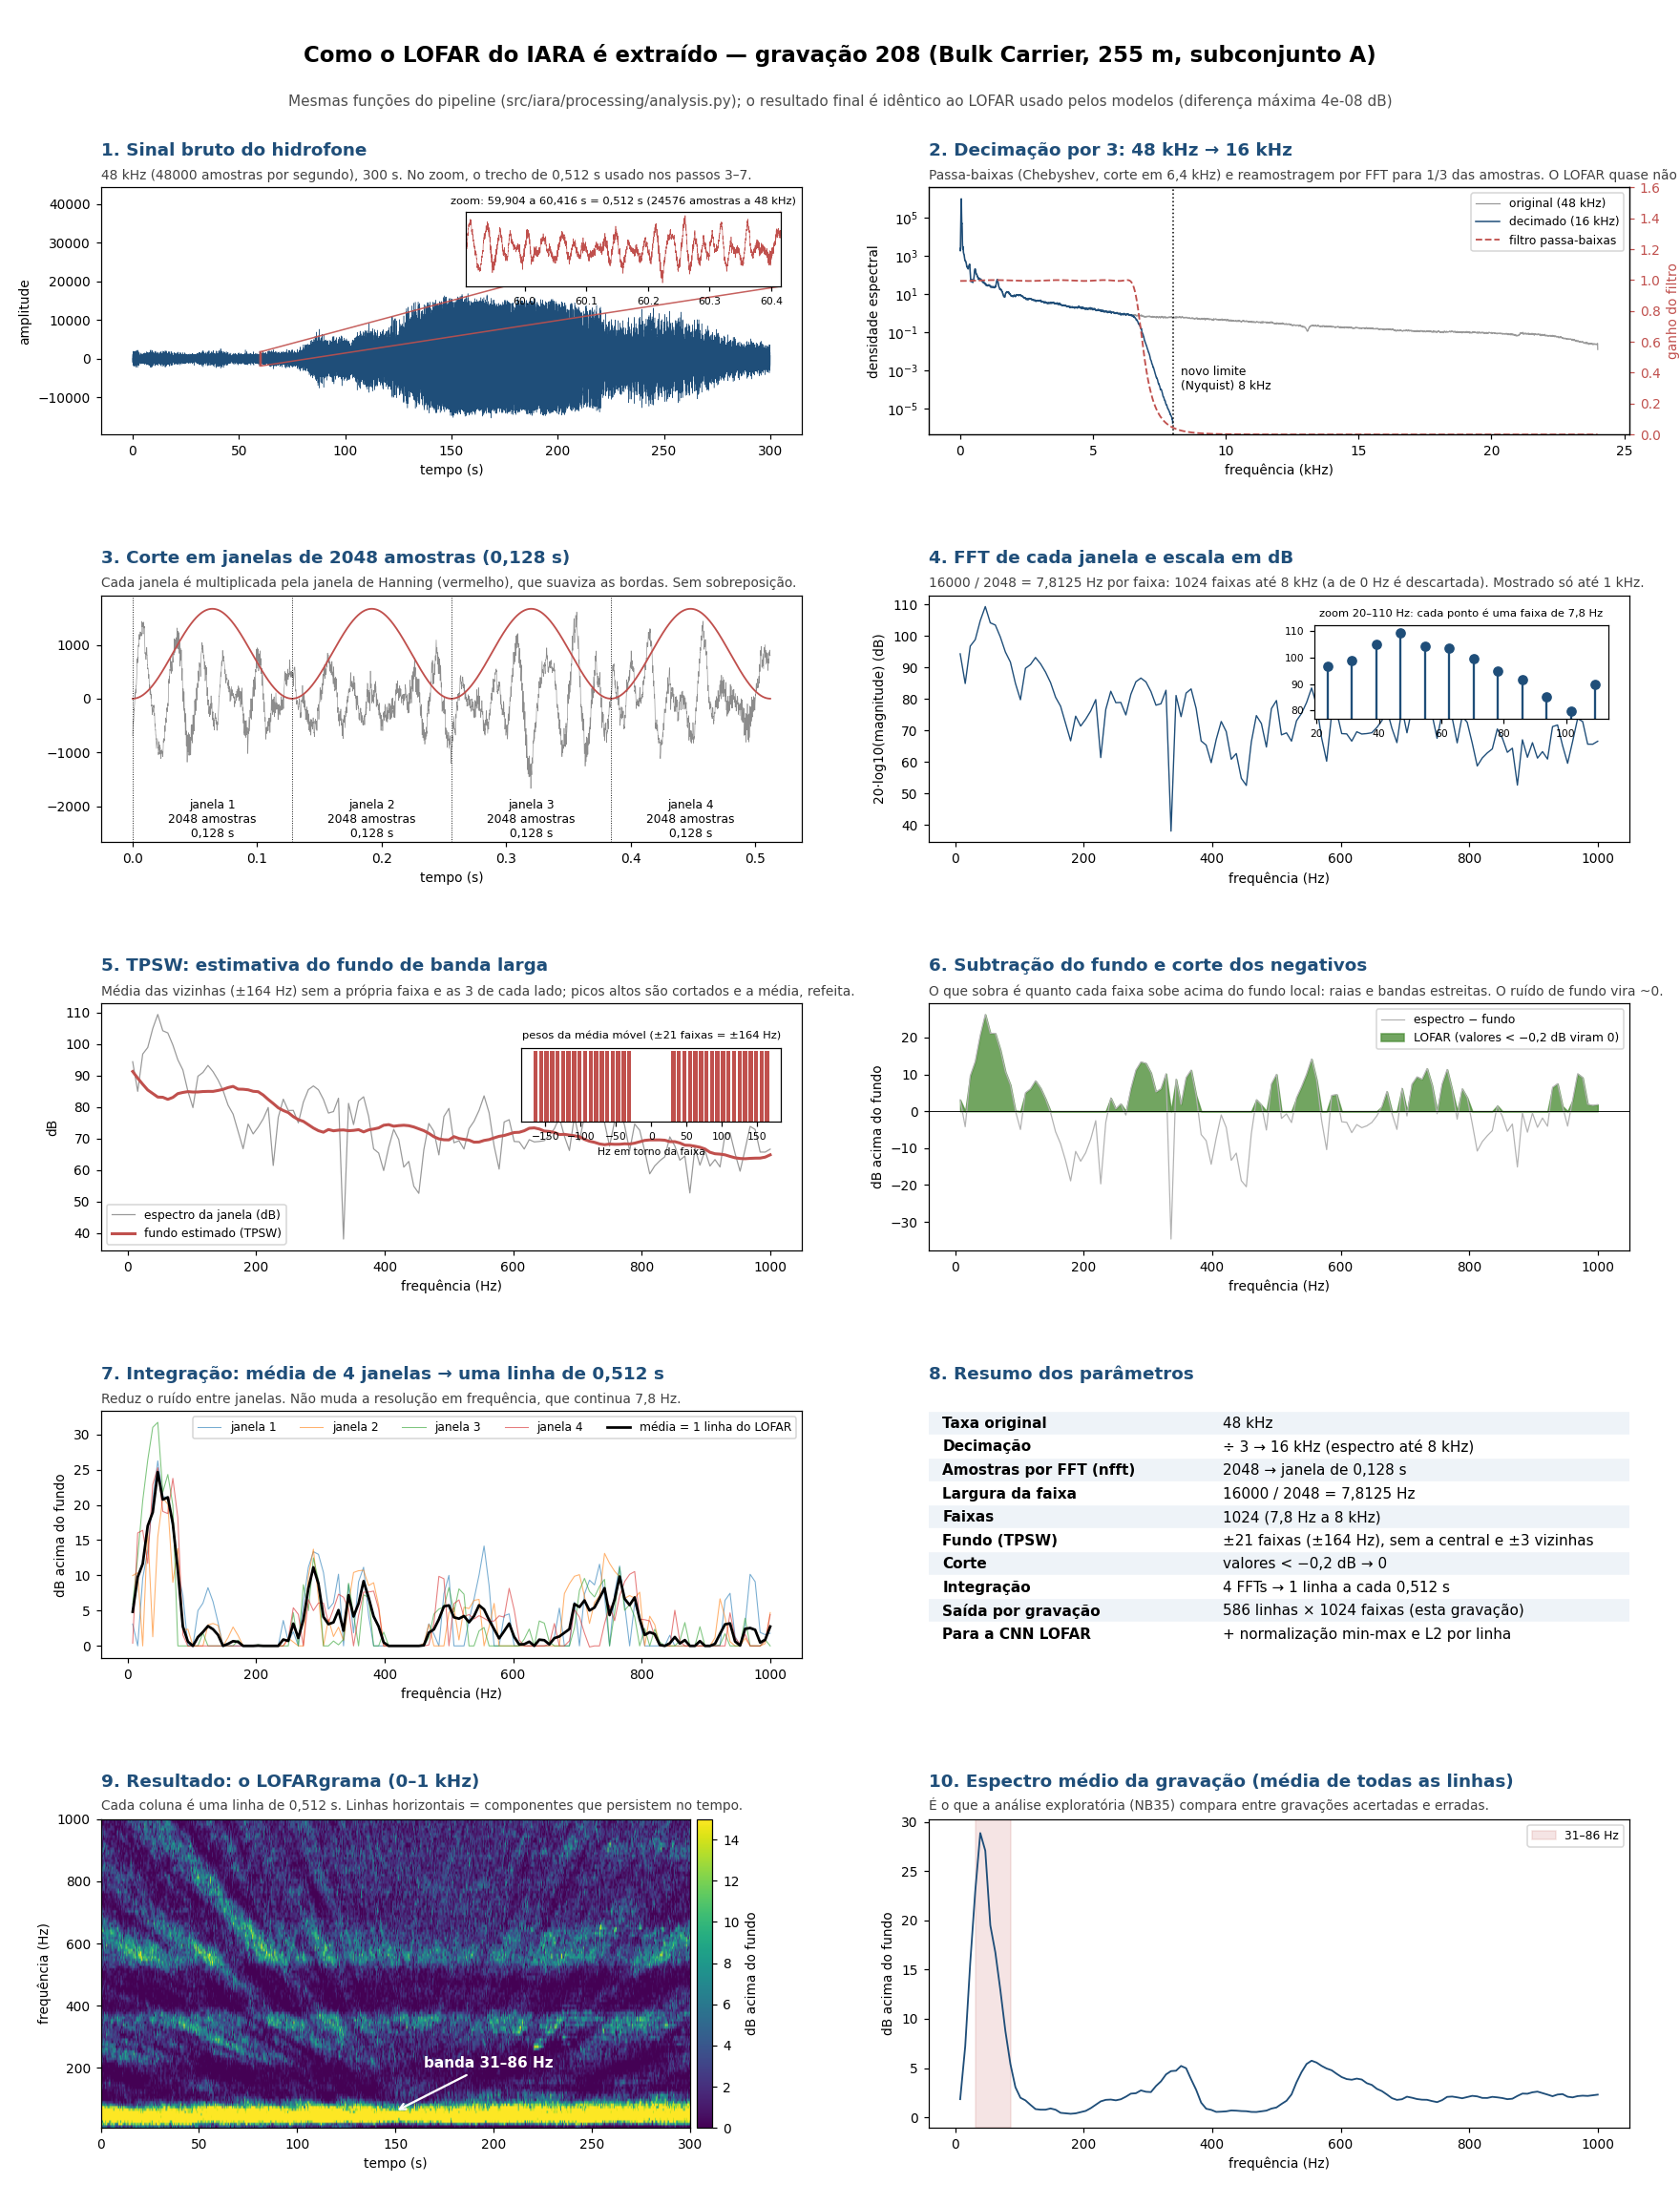
\includegraphics[height=0.82\textheight]{extracao_lofar.png}
        \column{0.6\textwidth}
        \begin{block}{\small Etapas}
            \scriptsize
            \begin{enumerate}
                \setlength{\itemsep}{1pt}
                \item Remoção da média e decimação $\times$3 (48 $\to$ 16 kHz; Chebyshev ordem 8, corte em 6,4 kHz, \texttt{filtfilt} e reamostragem por FFT).
                \item Janelas de Hann de 2048 amostras (0,128 s): faixas de 7,8125 Hz.
                \item Magnitude, 20$\cdot$log$_{10}$, remoção do fundo pelo TPSW (n = 21, p = 4, a = 2); valores abaixo de $-0{,}2$ viram 0.
                \item Média de 4 FFTs: uma linha a cada 0,512 s; para a CNN, min--max e L2 por linha.
            \end{enumerate}
            \vspace{0.05cm}
            O filtro atenua 6,4--8 kHz, mas o TPSW compensa (só vê a diferença para o fundo local).
        \end{block}
    \end{columns}
\end{frame}

\end{document}
